\documentclass{uflamon}          % classe base para a monografia

%==============================================================================
% Utilizacao de pacotes
\usepackage[T1]{fontenc}         % usa fontes postscript com acentos
%\usepackage{times}              % usa fonte times como default
\usepackage[brazil]{babel}       % hifenização e títulos em português do Brasil
\usepackage[utf8]{inputenc}     % permite edição direta com acentos
\usepackage{amsmath}             % pacote da AMS para Matemática Avançada
\usepackage{amssymb}             % símbolos extras da AMS
\usepackage{latexsym}            % símbolos extras do LaTeX
\usepackage{graphicx}            % para inserção de gráficos
\usepackage{listings}            % para inserção de código
\usepackage{fancyvrb}            % para inserção de saídas de comandos

\usepackage{colortbl} % frescuras em tabelas
\newcolumntype{L}{|>{\columncolor[gray]{0.9}}l|} %multicolunas boiolas

% cores para os links cruzados
\usepackage{color}
\definecolor{rltred}{rgb}{0.2,0,0}
\definecolor{rltgreen}{rgb}{0,0.2,0}
\definecolor{rltblue}{rgb}{0,0,0.2}

\usepackage[colorlinks=true,
	        urlcolor=rltblue,       % \href{...}{...} external (URL)
   	     filecolor=rltgreen,     % \href{...} local file
      	  linkcolor=rltred,       % \ref{...} and \pageref{...}
     		  citecolor=rltgreen,
    		  pdftitle={Simulação de algoritmo auto organizado para protocolo MAC em redes de sensores sem fio},
			  pdfauthor={Bruno Vitor Almeida Pinheiro},
           pdfsubject={Esse texto apresenta e discute protocolos de controle de acesso ao meio auto-organizados.},
           pdfkeywords={Protocolo de controle de acesso ao meio. 2. Auto-organização. 3. Redes de sensores sem fio. 4. RSSF. 5. MAC.}%
]{hyperref} % para referência cruzadas
%\usepackage{hyperref}            % para referência cruzadas
%\usepackage{subfigure}           % figuras dentro de figuras
\usepackage{caption2}            % remodelando o formato dos títulos de 
                                 % tabelas e figuras

% configuração padrão do listings   
\lstset{
   language=Java,
   extendedchars=true,
   tabsize=3,
   basicstyle=\footnotesize\ttfamily,
   stringstyle=\em,
   showstringspaces=false 
}

% para referências de acordo com a ABNT
% precisa instalar o abntex antes!!!
% http://abntex.codigolivre.org.br/
% comente se pretende usar outro padrão
\usepackage[alf,abnt-etal-cite=3,abnt-etal-list=0,abnt-etal-text=emph]{abntex2cite}


% redefinindo formatação de títulos de tabelas e figuras
\renewcommand{\captionfont}{\footnotesize}
\renewcommand{\captionlabelfont}{\footnotesize \bfseries}


%==============================================================================
% para os fãs do Word, descomente as linhas abaixo
%\sloppy %mais espaço entre as linhas
%\usepackage{identfirst} %identando-se a primeira linha de cada seção


%==============================================================================
% definido comandos na monografia - não é necessário na sua monografia 
% apenas para exemplificar a definição de novos comandos
\newcommand{\defs}[1]{\textsl{#1}}


% Especificando hifenizações que por ventura LaTeX não saiba fazer
% Por padrão 99,9% dos termos em português devem ser hifenizados corretamente.
\hyphenation{hardware software Li-nux am-bien-te diag-nos-ti-car coor-de-na-ção so-li-ci-ta-ção con-tro-le ou-tros
FAE-PE Recovery TelEduc Williams}

%==============================================================================
% Dados da monografia, capa: autor, titulo, banca, etc... - SUBSTITUA DE ACORDO
%==============================================================================
\author{Bruno Vitor Almeida Pinheiro}
\title{Simulação de algoritmo auto organizado para protocolo MAC em redes de sensores sem fio}
\date{2010}
\tipo{Monografia de Graduação  apresentada ao Departamento de Ciência da Computação 
da Universidade Federal de Lavras como parte das exigências do curso de 
Sistemas de Informação para obtenção do título de Bacharel em Sistemas de Informação.}
\areaconcentracao{Protocolos de Controle de Acesso ao Meio em Redes de Sensores Sem Fio}
\orientador{Prof. Tales}
% \coorientador{Prof. Silvino Santiago} % comente se não tiver coorientador
%\coorientadordois{Prof. Tiagão Meganha} % comente se não tiver coorientador
\bancaum{Prof. Juliana Galvani Greghi}
\bancadois{Prof. Marluce Rodrigues Pereira} % comente se sua banca tiver só um professor
%\bancatres{Fulanim de Sicrano}% comente se sua banca tiver só um professor
\defesa{25 de junho de 2010}
\palchaves{Protocolo de controle de acesso ao meio; Auto-organização; Redes de sensores sem fio; RSSF; MAC.}
\keywords{Medium access control protocol; Self-organization; Wireless sensor networks; WSN; MAC.}
%==============================================================================

%% dados para ficha catalográfica
% primeiro autor
\fcautor{Pinheiro, Bruno Vitor Almeida}
% autores, separados por vírgula
\fcautores{}

% % % % % % % % % % % % % % % % % % % % % % % % % % % % % % % % % % % % % % % % % % % % 
% dados para ficha catalográfica conforme modelo da BC-UFLA 
\fccatalogacao{Protocolo de controle de acesso ao meio. 2. Auto-organização. 3. Redes de sensores sem fio. 4. RSSF. 5. MAC. I. Pinheiro, B.V. A. II. Universidade Federal de Lavras.
  III. Fundação de Apoio ao Ensino, Pesquisa e Extensão.  
  IV. Simulação de algoritmo auto organizado para protocolo MAC em redes de sensores sem fio}
% % % % % % % % % % % % % % % % % % % % % % % % % % % % % % % % % % % % % % % % % % % % 

% classificação de acordo com a CDD, comente se não tiver isso.
\fcclasi{003.5}
\fcclasii{005.43}

\begin{document}
\maketitle

\dedic{Dedico esta monografia...}     % Dedicatórias
\thanks{Agradeço aos...}         % Agradecimentos

\pagestyle{ufla}
\pagenumbering{roman}

\tableofcontents                           % Sumário}
\listoffigures                             % Lista de Figuras
\listoftables                              % Lista de Tabelas

\resumo{Redes de sensores sem fio (RSSF) tem sido cada vez mais utilizadas em variados tipos de aplicações. Crescentes avanços tecnológicos nas áreas de sensores, radiotransmissores e outros equipamentos utilizados na construções de nós sensores dos quais são compostas essas redes tem reduzido a cada dia o custo de produção, bem como o de aquisição, desses equipamentos. Isso faz com que seja mais vantajoso a substituição dos nós que deixam de ser funcionais. Devido a isso e ao fato de que, em geral, nós sensores são alimentados por baterias e são dispostos muitas vezes em regiões que inviabilizam a substituição dessas baterias é importante desenvolver mecanismos que promovam um aumento na vida útil desses nós e, consequentemente, da rede como um todo. Os maiores consumidores de energia em nós sensores são os radiotransmissores. Através da utilização de protocolos de controle de acesso ao meio é possível manter controle sobre o ligamento e desligamento desses dispositivos, além de aumentar a eficiência de sua utilização por meio da eliminação ou diminuição da ocorrência de eventos que culminem na necessidade de retransmissão (por exemplo colisão de pacotes), dentre outros benefícios. Este trabalho contém informações gerais sobre as características das RSSF e cada uma das camadas da pilha de protocolos utilizados nesse tipo de rede. São apresentadas também informações relacionadas aos padrões de comunicação presentes nesse tipo de rede, bem como uma classificação dos protocolos MAC quanto à distribuição dos recursos para os nós, contendo exemplos de cada tipo de protocolo. E ao final são apresentados exemplos de protocolos MAC auto-organizados, seus mecanismos, suas vantagens e desvantagens.}%
%
\resumoingles{Wireless sensor networks (WSN) have been increasingly used in various types of applications. Increasing technological advancements in the areas of sensors, radio transceivers and other equipment used in the construction of sensor nodes that compose such networks has reduced production cost as well as the acquisition cost of such equipment. This makes it more interesting to replace the nodes that are no longer functional. Because of this and the fact that, in general, sensor nodes are powered by batteries and are often arranged in regions that prevent the replacement of these batteries, is important to develop mechanisms that promote an increase in the lifetime of these nodes and thus the network as a whole. The biggest consumers of energy in sensor nodes are the radio transceivers. Through the use of medium access control protocols (MAC) you can maintain control over the states (turned on/turned off) of such devices. In addition, it's possible to increasing the efficiency of its use through the elimination or reduction of the occurrence of events that culminate in the need for retransmission (e.g. collision of packets), and so forth. This work contains general information about the characteristics of wireless sensor networks and every layer of the protocol stack used in this type of network. It's also presented information related to communication patterns present in this type of network, and a classification of MAC protocols on the distribution of resources for the nodes, containing examples of each type of protocol. And at the end there are examples of self-organized MAC protocols, its mechanisms, advantages and disadvantages.}                         % Resumo (digite aqui o resumo)

\clearpage

%\pagestyle{ufla}
\pagenumbering{arabic}

%==============================================================================
% incluindo os capitulos

\section{Introdução}

Redes de sensores sem fio (RSSF) tem sido cada vez mais utilizadas em variados tipos de aplicações em diferentes tipos de ambientes, como no monitoramento de florestas para controle de incêndios, controle de irrigação em grandes plantações, controle de ventilação e condicionamento de ar em grandes edifícios, vigilância em áreas de interesse militar, automação industrial, etc. A cada dia surgem novas tecnologias em sensores, rádio transmissores e outros equipamentos utilizados na construção dos nós sensores que compõem esse tipo de rede, o que tem, cada vez mais, reduzido o custo para produção e, consequentemente, para a aquisição desses equipamentos.

Os nós sensores utilizados para a construção dessas redes são, em geral, alimentados por baterias, o que implica em sérias restrições ao seu tempo de vida útil \cite{Akyildiz2002a}. Considerando o fato de que a maioria das aplicações para esse tipo de rede é feita para utilização em ambientes que dificultam ou impossibilitam a substituição dessas baterias, torna-se necessário ou mais vantajoso substituir os próprios nós por novos. Embora o custo da substituição seja cada vez mais reduzido pelos avanços em tecnologia ainda é mais interessante fazer com que o tempo de vida da rede seja estendido através de mecanismos que possam reduzir o consumo de energia para se evitar uma alta frequência na necessidade de substituição dos nós sensores. Isso é possível através da utilização de protocolos eficientes no consumo de energia. 

\subsection{Motivação}

Em redes de sensores, o maior consumo de energia se dá na recepção e sobretudo na transmissão dos dados. Sendo assim é de suma importância garantir que a comunicação entre os nós sensores seja eficiente, evitando problemas que possam resultar na necessidade de retransmissão de pacotes(como no caso da colisão de pacotes por exemplo), bem como a recepção desnecessária de pacotes pelos nós da rede(\emph{overhearing}) ou mesmo a permanência dos receptores em atividade quando não há pacotes sendo enviados ao nó(\emph{idle listening}). Os responsáveis por evitar ou minimizar a ocorrência desses tipos de problemas são os protocolos de controle de acesso ao meio(MAC-\emph{Medium Access Control Protocols}). Esses protocolos determinam, dentre outras coisas, o momento em que cada nó pode começar ou não uma transmissão e os períodos em que o nó deve permanecer desligado ou ligado(ciclo de sono).

\subsection{Objetivos}

Esse trabalho tem por objetivo investigar mecanismos que promovam redução do consumo de energia em redes de sensores e aumentem seu tempo de vida útil para, ao final, propor um algoritmo que seja capaz de amenizar problemas causados por esses mecanismos, como o grande aumento no tempo de transmissão de pacotes entre pontos distantes na rede. Nas sessões seguintes serão apresentados a estrutura básica de uma rede de sensores, uma visão geral sobre as camadas que compõem a arquitetura dos nós. O foco da investigação são os protocolos da camada de controle de acesso ao meio (em inglês \emph{Medium Access Control - MAC}). Serão apresentados exemplos de protocolos existentes para essa camada incluindo uma classificação e exemplos de cada um deles. Também será apresentado um conceito de auto-organização e sua utilização nesses protocolos. O algoritmo proposto nesse trabalho deverá utilizar técnicas de auto-organização para promover uma organização na rede que possibilite o aumento da velocidade de comunicação entre nós selecionados ao passo que aumenta os períodos de inatividades dos demais nós. Espera-se com isso promover redução do tempo de transmissão de pacotes entre pontos distantes ao fazer com que esses passem necessariamente pelos nós selecionados no passo anterior. 
\section{Motivação}

Em redes de sensores, o maior consumo de energia se dá na recepção e sobretudo na transmissão dos dados. Sendo assim é de suma importância garantir que a comunicação entre os nós sensores seja eficiente, evitando problemas que possam resultar na necessidade de retransmissão de pacotes(como no caso da colisão de pacotes por exemplo), bem como a recepção desnecessária de pacotes pelos nós da rede(\emph{overhearing}) ou mesmo a permanência dos receptores em atividade quando não há pacotes sendo enviados ao nó(\emph{idle listening}). Os responsáveis por evitar ou minimizar a ocorrência desses tipos de problemas são os protocolos de controle de acesso ao meio(MAC-\emph{Medium Access Control Protocols}). Esses protocolos determinam, dentre outras coisas, o momento em que cada nó pode começar ou não uma transmissão e os períodos em que o nó deve permanecer desligado ou ligado(ciclo de sono).
\section{Objetivos}

Este trabalho tem por objetivo apresentar a estrutura básica de uma rede de sensores, uma visão geral sobre as camadas que compõem a rede, vários exemplos de protocolos MAC incluindo uma classificação desses protocolos e exemplos de cada um dos tipos apresentados para ao final apresentas uma proposta de algoritmo para protocolo MAC que utilizará técnicas de auto-organização para promover uma organização na rede que possibilite o aumento da eficiência na comunicação entre os nós pertencentes a ela, além de reduzir o consumo de energia através do aumento na velocidade de comunicação o que possibilitará um aumento na duração dos períodos de sono(quando o nó permanece desligado) dos nós.
\chapter{Redes de Sensores Sem Fio}

Graças aos avanços tecnológicos na área de comunicação sem fio e de eletrônicos tem sido cada vez mais fácil desenvolver nós sensores multifuncionais de baixo custo e consumo de energia capazes de se comunicar a curtas distâncias. Disso surge a ideia da criação de redes de sensores sem fio.

Redes de sensores sem fio(RSSF) são redes compostas por um grande número de nós sensores densamente distribuídos dentro de um fenômeno ou próximo a ele, cujas posições não precisam ser predeterminadas e que trabalham de forma cooperativa para a realização de tarefas. Isso possibilita a distribuição aleatória em regiões inacessíveis, porém também torna necessária a criação de protocolos e algoritmos com capacidade de auto organização\cite{Akyildiz2002}.

\begin{figure}[!htb]
\centering
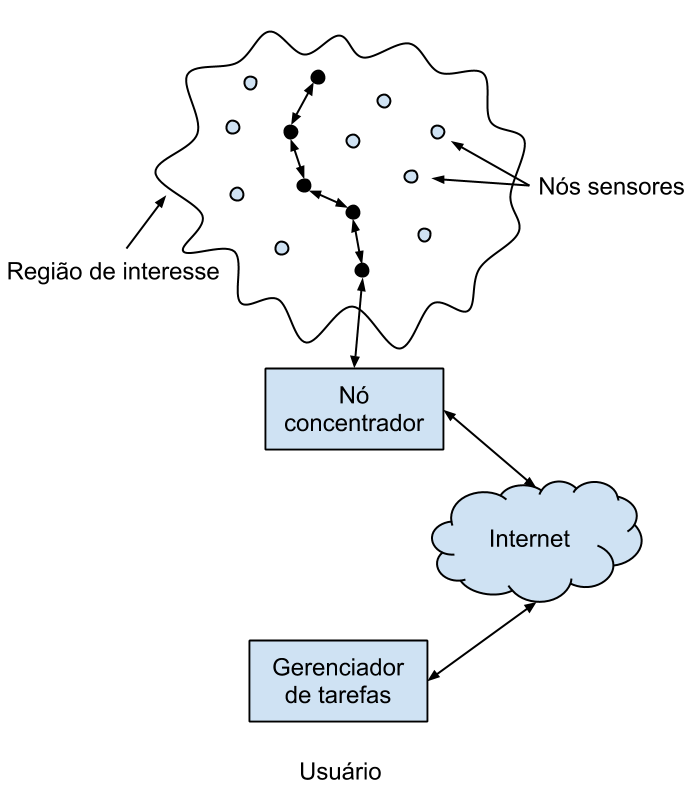
\includegraphics[width=200px,height=280px]{./Pictures/SensorNodesScatteredInASensorField.png}
% SensorNodesScatteredInASensorField.png: 816x1056 pixel, 96dpi, 21.59x27.94 cm, bb=0 0 612 792
% pdfLaTeX aceita figuras no formato PNG, JPG ou PDF
% figuras vetoriais podem ser exportadas para eps e depois convertidas para pdf usando epstopdf
\caption{Exemplo da distribuição dos nós de uma RSSF em uma região de interesse} %legenda
\label{fig:snsf} %rotulo para refencia
\end{figure}

A Figura~\ref{fig:snsf} mostra como os nós de uma rede de sensores ficam distribuídos em uma região de interesse(\textit{sensor field}). Cada um dos nós(\textit{sensor nodes}) coleta dados do ambiente e pode roteá-los até o nó \textit{sink} (nó que reúne as informações da rede) e este pode comunicar-se com o gerenciador de tarefas por meio da internet ou de satélites.

Romer e Matter(2004)\cite{Romer2004} definem RSSF como redes \textit{ad hoc} de larga escala, \textit{multi-hop}, não particionada composta por nós sensores, em sua maioria imóveis, largamente homogêneos, pequenos e com recursos limitados, randomicamente distribuídos em uma área de interesse.

Karl e Willing(2005)\cite{Karl2005} apresentam uma definição de redes \textit{ad hoc} como redes configuradas para, literalmente, atender a um propósito específico e a necessidades específicas de comunicação. \cite{Karl2005} apresenta também uma definição para \textit{Mobile Ad Hoc Networks}(MANET) que seria uma rede \textit{ad hoc} associada à comunicação sem fio(\textit{wireless}) e à mobilidade dos nós participantes. 


Listadas abixo estão algumas diferenças significativas entre redes \textit{ad hoc} e RSSF:
\begin{itemize} 
	\item O número de nós sensores em RSSF pode ser de uma ordem de magnitude muio acima da encontrada em redes \textit{ad hoc}\cite{Akyildiz2002}.
	\item MANET são utilizadas em aplicações como comunicação por voz ou acesso a infraestrutura remota necessitando assim de equipamentos robustos o suficiente para suportar esse tipo de aplicações ao contrário de RSSFs que são compostas por equipamentos bem mais simples e limitados\cite{Karl2005}. 
	\item RSSF são capazes de comportar variados cenários de aplicação, devido ao grande número de combinações possíveis de tecnologias de comunicação, computação e sensores. Por exemplo conseguindo trabalhar em diversas e variáveis densidades, o que irá requerer o uso de diferentes protocolos ou protocolos adaptativos. Tal flexibilidade existe também em MANET, porém em um nível bastante reduzido\cite{Karl2005}. 
	\item A densidade das RSSF é bem maior que a encontrada nas MANET\cite{Akyildiz2002}.
	\item Nós sensores de uma RSSF são suscetíveis a erros e a topologia da rede muda com frequência\cite{Akyildiz2002}. 
	\item Em RSSF predomina o paradigma de comunicação \textit{broadcast}, ao contrário do que predomina em redes \textit{ad hoc} que é a comunicação \textit{point-to-point}.
	\item Nós de uma RSSF podem não possuir uma identificação global devido ao grande número de nós sensores, pois isso causaria um grande \textit{overhead}.
\end{itemize} 

% +++++++++++++++++++++++++++++++++++++++++++++++++++++++++++++++++++++++++++++++++++++++++++++++++++++++++++++++++++++
\section{Características de RSSF} \label{sec:featuresRSSF}
% +++++++++++++++++++++++++++++++++++++++++++++++++++++++++++++++++++++++++++++++++++++++++++++++++++++++++++++++++++++

Há inúmeros problemas encontrados nesse tipo de redes e um número igualmente grande de soluções propostas para cada um desses problemas. De maneira geral, nós de uma rede de sensores sem fio são alimentados por baterias e, consequentemente, possuem um tempo de vida útil consideravelmente limitado, tendo em vista que, na maioria das utilizações desse tipo de rede não é possível fazer a substituição das baterias. Tal asserção baseia-se no fato que esse tipo de solução, dadas as suas limitações, só seria empregada em casos onde outras soluções mais simples ou eficientes não pudessem ser empregadas, como no monitoramento de áreas de difícil acesso, por exemplo, o interior de florestas ou áreas de desastre. 

Algumas das principais características que uma RSSF deve apresentar são:
 \begin{itemize}
 \item \textbf{Tolerância a falhas:} Alguns nós da rede podem deixar de funcionar devido a vários fatores como o fim de suas baterias ou dano físico. Tolerância a falhas é a capacidade de manter a rede de sensores funcionando sem interrupções devido a falhas em nós sensores\cite{Srisathapornphat2001,Hoblos2000}.
 \item \textbf{Escalabilidade:} O número de nós distribuídos para o estudo de um fenômeno pode atingir valores muito elevados(ordem de centenas de milhares ou mais). Além disso pode existir um número muito grande de nós em uma área muito pequena(alta densidade). Devem ser desenvolvidos mecanismos e protocolos capazes de trabalhar com esse número de nós.
 \item \textbf{Tempo de vida:} Na maioria dos cenários de utilização de RSSF limitam ou impossibilitam a substituição de baterias nos nós\cite{Karl2005}. Ainda assim, espera-se que uma rede de sensores permaneça em funcionamento por um determinado período de tempo necessário à realização de uma missão ou o maior tempo possível. Portanto, torna-se evidente a necessidade de fazer com que a rede opere de modo eficiente em relação ao consumo de energia.
 \item \textbf{Programabilidade:} Os nós de uma rede de sensores devem processar informações, mas além disso precisam ser capazes de se adaptar a mudanças em suas tarefas. Eles devem ser programáveis e sua programação deve ser passível de alterações mesmo quando em operação para atender a novas tarefas que venham a se tornar importantes\cite{Karl2005}.
 \item \textbf{Manutenibilidade:} Com o passar do tempo podem ocorrer mudanças tanto no ambiente como na rede de sensores. Essas mudanças podem ser causadas por vários fatores, como falha de nós ou surgimento de novas tarefas. A rede deve adaptar-se a essas mudanças e monitorar o seu próprio estado, fazendo as alterações nos parâmetros operacionais quando necessário, por exemplo reduzindo a qualidade do serviço quando o nível de energia estiver baixo. Ela poderia interagir com mecanismos externos de manutenção para garantir a continuidade de sua operação a um nível mínimo de qualidade necessário por uma maior período de tempo\cite{Mainwaring2002}.
 \end{itemize}

%=====================================================================
\section{Protocolos em RSSF} 
%==============================

A pilha de protocolos usados em redes de sensores sem fio são responsáveis por prover comunicação eficiente, em termos de energia e roteamento, no meio sem fio, integração entre dados e protocolos de rede e promover o esforço cooperativo dos nós sensores \cite{Akyildiz2002}. Os protocolos estão distribuídos entre as camadas da rede. Uma descrição de cada camada é apresentada em \cite{Akyildiz2002} e descrita resumidamente a seguir. A Figura~\ref{fig:protocolStack} é uma representação da pilha de protocolos.

\begin{figure}[!htb]
\centering
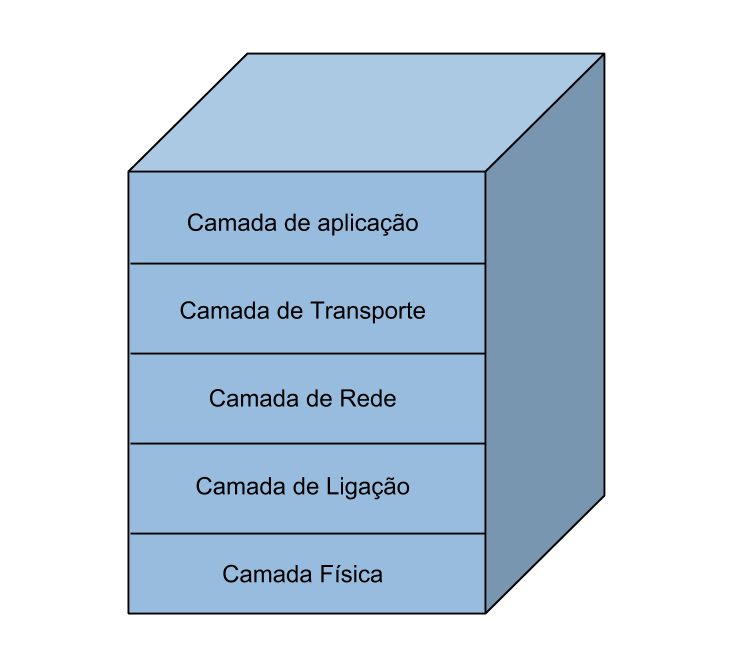
\includegraphics[width=230px,height=280px]{./Pictures/ProtocolStack.png}
% SensorNodesScatteredInASensorField.png: 816x1056 pixel, 96dpi, 21.59x27.94 cm, bb=0 0 612 792
% pdfLaTeX aceita figuras no formato PNG, JPG ou PDF
% figuras vetoriais podem ser exportadas para eps e depois convertidas para pdf usando epstopdf
\caption{Pilha de protocolos em redes de sensores sem fio} %legenda
\label{fig:protocolStack} %rotulo para refencia
\end{figure}


 %---------------------------------------------------------------------
 \subsection{Camada física (\textit{physical layer})} 
 %------------------------------------------------------

 A camada física é responsável por selecionar a frequência, geração de frequência portadora\textit{carrier frequency generation}, detecção de sinais, modulação e encriptação de dados. O custo, tanto em termos de consumo de energia quanto em complexidade de implementação, da comunicação sem fio a longas distâncias é muito elevado. Em redes de sensores sem fio, a minimização do consumo de energia tem importância significativa na propagação e nos efeitos que causam desvanecimento do sinal. Em geral, a potência necessária para transmitir um sinal a uma distância \textit{$d$} é diretamente proporcional a \textit{$d^{n}$}, sendo 2 <= \textit{n} < 4. n é próximo de 4 para antenas muito baixas e canais muito próximas do chão \cite{Pottie2000} citado por \cite{Akyildiz2002}.
 
 %---------------------------------------------------------------------
 \subsection{Camada de ligação de dados(\textit{Data Link Layer}) }
 %--------------------------------------------------------------------
 
 Camada de ligação de dados é a camada responsável por multiplexação de fluxos de dados(\textit{data streams}), detecção de quadros de dados(\textit{data frames}), acesso ao meio(\textit{medium access}) e controle de erros(\textit{error control}).
 
 \subsubsection{Protocolos de controle de acesso ao meio}
 
 Protocolos de controle de acesso ao meio (\textit{Medium Access Control Protocols}) atuam nessa camada. Eles coordenam o acesso ao meio físico por nós ativos. Esses protocolos são de grande importância, uma vez que o canal de comunicação sem fio (\textit{wireless}) é inerentemente propenso a erros, além de outros problemas específicos desse tipo de rede, tais como: o problema do terminal escondido (\textit{hidden-terminal}), problema do terminal exposto(\textit{exposed-terminal}) e efeitos do desvanecimento de sinal (\textit{signal fading effects}) Kumar et. al. (2006) \cite{Kumar06mediumaccess}. Esses protocolos serão abordados mais detalhadamente na sessão ~\ref{sec:macProtocols}.

 
 %---------------------------------------------------------------------
 \subsection{Camada de rede( \textit{Network layer})} 
 %------------------------------------------------------
 
 Técnicas convencionais de roteamento não são aplicáveis às características específicas desse tipo de redes (algumas delas podem ser encontradas na sessão ~\ref{sec:featuresRSSF}). A camada de rede em redes desenvolvida de acordo com as seguintes restrições \cite{Guerses2005}:
 
 \begin{itemize}
 \item \textbf{Não há um identificador global}, devido a existência de poucos dados de eventos e um grande número de nós.
 \item \textbf{Eficiência de energia} é necessária para aumentar o tempo de vida da rede.
 \item \textbf{Descoberta de rotas auto organizável} para lidar com mudanças na topologia da rede.
 \item \textbf{Modelo de distribuição de dados} pode ser dos tipos \cite{Tilak02ataxonomy}:
 \subitem \textbf{contínuo} - sensores entregam os dados continuamente;
 \subitem \textbf{dirigido a eventos} - sensores entregam dados ao detectarem um evento de interesse;
 \subitem \textbf{dirigido a consultas} - os nós entregam dados a partir da uma solicitação iniciada pelo observador;
 \item \textbf{Processamento em rede} por meio da utilização de ``funções de agregação'' é um requisito para comunicação eficiente em termos de energia;
 \item \textbf{Comunicação local inter sensor} é um requisito para aplicações, bem como para o processamento em rede;
 \item \textbf{Qualidade de serviço} (largura de banda, quantidade de erros e latência) deve atenter aos requisitos das aplicações; 
 
 \end{itemize}

 %---------------------------------------------------------------------
 \subsection{Camada de transporte} 
 %------------------------------------------------------
 
 Muitas aplicações de redes de sensores sem fio requerem mecanismos de controle de congestionamento para regular a quantidade de tráfego injetada na rede com o objetivo de evitar perda de pacotes e para atribuir confiabilidade à entrega de pacotes e eventos \cite{RaSaGu2008-InCol}. Em várias aplicações há nós responsáveis por capturar informações críticas e enviá-las a um nó concentrador (\textit{sink node}) \cite{RaSaGu2008-InCol}. Os protocolos dessa camada são desenvolvidos para atender a essas restrições e garantir que os pacotes sejam enviados e alcancem seus destinos corretamente.

 \subsection{Camada de aplicação}
 
 Segundo Alkyildniz et. al. (2002), embora haja muitas aplicações propostas para redes de sensores, potenciais protocolos para a camada de aplicação permanecem em uma região altamente inexplorada. Esses protocolos possibilitam a interação entre a camada de aplicação e as camadas inferiores. Há três protocolos mais comuns utilizados nessa camada. 
 
 \begin{itemize}
 \item \textbf{Protocolo de gerenciamento de sensores:} protocolos de gerenciamento na camada de aplicação tornam o \textit{hardware} e o \textit{software} das camadas inferiores transparentes para aplicações de gerenciamento de redes de sensores.
 \item \textbf{Protocolo de atribuição de tarefas e anúncio de dados (\textit{data advertisement}):} utilizado para atribuição de tarefas aos nós e também para comunicação de detecção de eventos pelos nós.
 \item \textbf{Protocolo de requisição (\textit{sensor query}) e disseminação de dados:} utilizados para fazer consultas ou requisições de dados aos sensores e devolução das respectivas respostas.
 \end{itemize}


\section{Controle de acesso ao meio}
\label{sec:macProtocols}

Protocolos de controle de acesso ao meio(MAC) são a primeira camada de protocolo acima da camada física e são responsáveis por prover endereçamento e acesso ao canal de comunicação. Segundo Karl and Willig(2005)\cite{Karl2005},a tarefa principal de qualquer protocolo MAC é regular o acesso de um número de nós a um meio de comunicação compartilhado, de tal modo que os requisitos de performance de cada aplicação sejam satisfeitos.

Nós sensores são alimentados por baterias, o que faz com que o consumo de energia seja uma restrição muito forte a ser tratada. Crescentes avanços tecnológicos tem tornado o custo de produção dos nós cada vez menor. Em razão disso, tem se tornado cada vez mais vantajoso substituir os nós ao invés de trocar suas baterias, tendo em vista que, na maioria dos casos, eles são inseridos em ambientes que dificultam ou mesmo impossibilitam o procedimento de troca. 

Segundo Ye (2002)\cite{Ye2002}, para desenvolver protocolos para redes de sensores, é preciso considerar como atributos principais a serem alcançados: eficiência no consumo de energia para aumentar a vida útil da rede, dado às dificuldades de substituição das baterias; escalabilidade para adaptação a mudanças no tamanho, densidade e topologia da rede, uma vez que alguns nós da rede irão morrer com o passar do tempo, novos nós podem ser inseridos na rede mais tarde, além disso, alguns nós podem se mover para locais diferentes. Outros atributos como justiça na distribuição de recursos(por exemplo o meio de comunicação), latência, e ritmo de transferência de dados que são tidos como principais em outros tipos de redes sem fio são aqui tidos como secundários.

%---------------------------------------------------------------------
\subsection{Padrões de comunicação em RSSFs}
\label{sec:comnPatt}
%-------------------------------------------
 
Segundo Demirkol et. al.(2006) \cite{Demirkol2006}, os tipos de padrões de comunicação em RSSFs determinam o comportamento do tráfego de dados na redes de sensores que deve ser tratado pelos protocolos de controle de acesso ao meio(MAC). 

Kulkarni (2004)\cite{Kulkarni2004} define três tipos de comunicação em redes de sensores sem fio: \textit{broadcast}, \textit{convergecast}, \textit{local gossip}. O padrão \textit{broadcast} é geralmente utilizados por estações base (\textit{sink nodes}) para trasmitir informações para todos os nós da rede. Pacotes enviados em \textit{broadcast} podem conter requisições por informações dos sensores, atualizações do programa para os nós sensores, pacotes de controle para todo o sistema, etc. \textit{Local gossip} ocorre quando um nó sensor detecta um evento e o comunica a cada um de seus vizinhos localmente (dentro do alcance de seu radiotransmissor). Após um grupo de nós detectar um evento, é necessário comunicá-lo ao centro de informações, esse padrão de comunicação é chamado \textit{convergecast} (quando um grupo de sensores se comunica com um sensor específico).

%---------------------------------------------------------------------
\subsection{Classificação de Protocolos de Controle de Acesso ao Meio}
%---------------------------------------------------------------------

A cada dia surgem novas propostas de protocolos MAC que utilizam diferentes técnicas para alcançar melhores resultados em termos de consumo de energia, latência, qualidade de serviço, etc., de acordo com as necessidades de cada aplicação. Chandra \cite{Chandra_2wireless} classifica os protocolos MAC nas seguintes classes: protocolos de atribuição fixa, protocolos de atribuição por demanda e protocolos de acesso aleatório.

 \subsubsection{Protocolos de atribuição fixa} 
 
 Cada nó recebe uma porção do recursos por um período de tempo considerado longo (da ordem de minutos, horas, ou mesmo maior) e pode utilizá-los de maneira exclusiva naquele período de tempo, ou seja, somente o nó ao qual um recurso foi atribuído pode acessar esse recurso no espaço de tempo que foi para ele reservado. 
 
 A atribuição desses recursos não é feita de maneira permanente devido à necessidade de adaptação a possíveis alterações na topologia da rede (quando ocorre a morte, inserção ou movimentação de nós na rede, por exemplo). Esse tipo de atribuição feito por períodos consideravelmente longos pode causar efeitos negativos à característica de escalabilidade da rede. 
 
 Como exemplos desse tipo de protocolo tem-se o \textit{Time Divided Multiple Access} (TDMA) \cite{Kulkarni2004} onde o tempo de uso dos recursos é dividido em \textit{slots} que são atribuídos aos nós da rede, \textit{Frequency Division Multiple Access} (FDMA) onde a banda de frequência e dividida em vários sub-canais (faixas de frequência) que são atribuídos aos nós da rede \cite{Arms_frequencyagile}.
	
 \subsubsection{Protocolos de atribuição por demanda} 
 
 Nesse tipo de protocolo, ao contrário dos protocolos de atribuição fixa, os recursos são distribuídos entre os nós por um período de tempo relativamente curto (da ordem de dezenas de milissegundos), geralmente o tempo necessário para o envio de um conjunto de pacotes de dados. Caso um nó necessite utilizar algum recurso, este deve fazer uma solicitação a um nó central que seja responsável por coordenar o uso de tal recurso, que por sua vez retorna a confirmação ou não da alocação do recurso e, em caso positivo, uma descrição do recurso alocado. Após essa negociação, o nó solicitante poderá utilizar o recurso de maneira exclusiva. A comunicação para requisição de um recurso é, em geral, feita através de protocolos de acesso aleatório em canais dedicados. Uma outra possibilidade, é deixar a estação central organizar os nós associados a ela. 
 
 Uma restrição no uso desse tipo de organização é que a estação central precisa estar ligada todo o tempo e, portanto, não pode ter restrições de energia. Esse tipo de protocolos pode ser ainda dividido em duas outras subcategorias: protocolos centralizados(onde exista apenas uma estação central) e protocolos distribuídos (onde exista várias estações centrais, cada uma responsável pela alocação dos recursos em uma determinada região da rede). 
 
 Como exemplo temos o \textit{Predictive Demand Assignment Multiple Access} (PRDAMA) \cite{Jiang_apredictive}, que aloca recursos de largura de banda através de estimativa da variação positiva do tráfego da internet para predeterminar a necessidade de recursos das estações.

 \subsubsection{Protocolos de acesso aleatório}	

 Em protocolos desse tipo não há coordenação para o uso de recursos. Cada nó que necessite de um recurso (como o meio de comunicação, por exemplo), deve verificar se o recurso está disponível ou tentar acessá-lo diretamente podendo considerar algum parâmetro aleatório, por exemplo, após aguardar um tempo aleatório ou relacionado com o tempo de chegada de pacotes randômicos. Caso o recurso esteja indisponível ou inacessível repete-se o procedimento de acordo com novos valores aleatórios. 
 
 Um exemplo desse tipo de protocolo é o ALOHA \cite{Baccelli06analoha}, que permite que os nós enviem pacotes no momento em que existam pacotes a serem enviados. Em seguida eles devem aguardar a confirmação do recebimento dos pacotes e, em caso positivo enviar o pacote seguinte (caso haja) ou, no caso contrário, reenviar o pacote.
 
\section{Auto-Organização em RSSF}

 Auto-organização é um processo pelo qual estrutura e funcionalidade (padrão) em nível global de um sistema emergem unicamente de numerosas interações entre componentes de baixo nível de um sistema sem qualquer controle externo ou centralizado. Os componentes do sistema interagem em um contexto local por meio de comunicação direta ou observações ambientais sem referência a um padrão global \cite{Dressler2008}.
 
 \subsection{Protocolos MAC auto-organizáveis}
 
 A utilização de auto-organização em redes de sensores sem fio possibilita ganhos em certos atributos dessas redes, como escalabilidade, consumo de energia, tolerância a falhas, etc. Em protocolos de acesso ao meio, auto-organização é utilizada em mecanismos como: atribuição de recursos aos nós \cite{Dressler2008}, determinação de ciclos de sono%
 % FOOTNOTE begin 
 \footnote{Com o objetivo de aumentar o tempo de vida útil das RSSF são utilizados ciclos de sono (\textit{sleep-wakeup cycle} ou \textit{duty cycle}) onde cada nó é ligado apenas por um curto período de tempo (\textit{wakeup}) e então desligado novamente (\textit{sleep}). A utilização desses ciclos pode aumentar a vida útil das RSSF, devido à redução do consumo de energia durante o período de sono \textit{sleep}, de poucos dias para vários meses ou mesmo anos dependendo da razão entre o tempo em que o nó permanece ligado e o tempo em que permanece desligado.}
 % FOOTNOTE end
 \cite{Halkes:2005}, roteamento de pacotes, etc. Existem muitos exemplos de protocolos de controle de acesso ao meio que utilizam esse tipo de organização para diversos fins, abaixo estão apresentados alguns desses protocolos e o modo como a auto-organização é empregada neles.
 
 \subsubsection{WiseMAC}
 
 WiseMAC \cite{El-Hoiydi2004} é baseado em técnicas de amostragem de preâmbulo ??ESSA É UMA CITAÇÃO DENTRO DO ARTIGO, DEVO COLOCAR? \cite{El-Hoiydi2002}??. Através da verificação periódica do meio em busca de atividades de comunicação. Tal verificação consiste em uma varredura de curta duração do canal de rádio. Cada nó verifica o meio com um mesmo período constante \textit{Tw} (~\ref{fig:wisemac}). Se o meio está ocupado, o nó sensor continua a ouvi-lo até receber um quadro de dados ou até o meio ficar desocupado novamente. Antes de cada quadro de dados ser enviado, o ponto de acesso (\textit{access point}) envia um preâmbulo com a mesma duração do período de verificação para garantir que o receptor esteja acordado no momento em que o quadro de dados for enviado. Essa técnica promove um baixo consumo de energia quando o canal está desocupado, porém tem como desvantagem o fato de que os preâmbulos utilizados podem causar limitações à velocidade de transmissão entre pontos distantes e maior consumo de energia devido a sobrecarga nos receptores e ao fato de todos os nós permanecerem ouvindo essa transmissão (\textit{overhearing}). Um ganho considerável é conseguido ao fazer com que os pontos de acesso conheçam os ciclos de verificação dos outros nós pois ele poderá iniciar transmissões somente no momento em que os outros nós estarão ouvindo.
 
\begin{figure}[!htb]
\centering
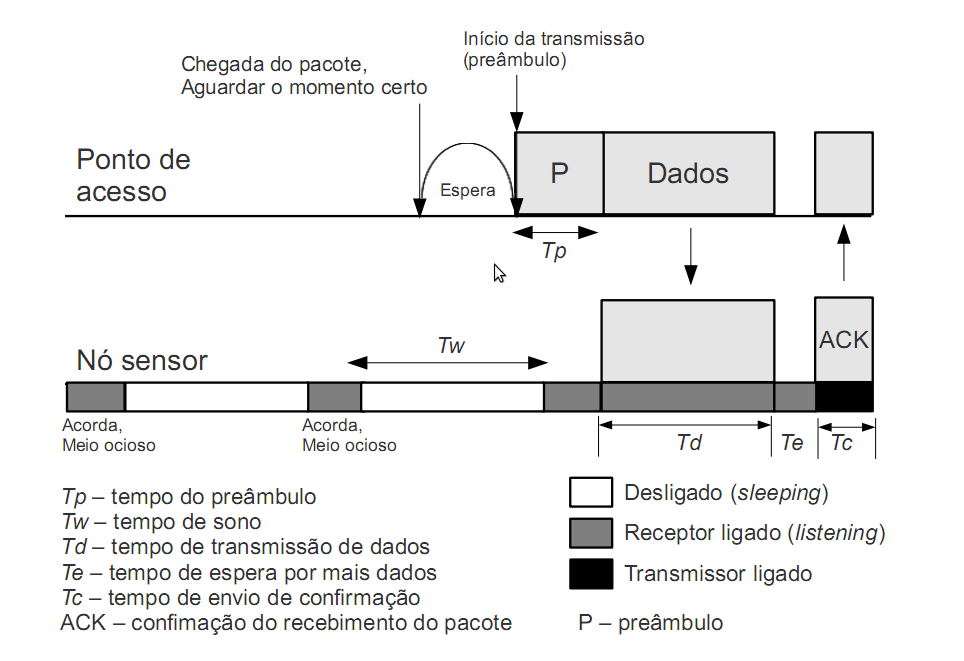
\includegraphics[width=340px,height=220px]{./Pictures/wisemac.png}
% SensorNodesScatteredInASensorField.png: 816x1056 pixel, 96dpi, 21.59x27.94 cm, bb=0 0 612 792
% pdfLaTeX aceita figuras no formato PNG, JPG ou PDF
% figuras vetoriais podem ser exportadas para eps e depois convertidas para pdf usando epstopdf
\caption{Funcionamento do WiseMAC \cite{El-Hoiydi2004}} %legenda
\label{fig:wisemac} %rotulo para refencia
\end{figure}

 \subsubsection{S-MAC}
 
 Sensor-MAC (S-MAC) [REF HERE] foi desenvolvido para ter primordialmente baixo consumo de energia, além disso conseguiu-se também boa escalabilidade e baixo número de colisões. Para conseguir esse resultados foram tratados os seguintes problemas identificados pelo autor como responsáveis pelo consumo excessivo de energia na rede: colisões de pacotes, que causam a retransmissão desses pacotes e consequente consumo extra de energia além de aumentar a latência na rede; \textit{overhearing}, que acontece quando os nós recebem pacotes que não são destinados a eles; excesso (\textit{overhead}) de pacotes de controle; e \textit{idle listening}, quando um nó permanece em modo de recepção aguardando por pacotes que não são enviados.

 Para alcançar esses resultados foi adotado um padrão ciclos de sono com períodos maiores de sono (nó desligado) e períodos de atividade curtos. Auto-organização está presente na sincronização dos períodos de atividade/sono dos nós em uma vizinhança, fazendo com que os nós adotem um mesmo cronograma de funcionamento. Isso possibilita que eles possam se comunicar e transmitir informações com eficiência apesar do maior tempo de inatividade. Além disso pode-se reduzir o tamanho dos preâmbulos%
 % PREÂMBULO 
 \footnote{Preâmbulo é um fluxo de dados utilizado para comunicar a intenção de transmitir. Tem duração variável de acordo com o período de sono, pois é preciso garantir que o destinatário receba esse preâmbulo e identifique-se como receptor dos pacotes de dados que serão enviados em seguida.}
 %
 pois tem-se uma garantia de que o(s) nó(s) aos quais os dados se destinam serão acordados no mesmo momento (ou em um momento muito próximo) em que aquele que deseja transmitir.
 
 Como desvantagem desse protocolo pode-se destacar que a sincronização dos ciclos de sono se dá entre um certo número de nós de uma região da rede e os nós que ficam no limiar entre duas regiões devem sincronizar-se com ambas as regiões (~\ref{fig:SmacSynch}). Isso faz com que o consumo de energia desses nós seja maior, reduzindo-se assim o seu tempo de vida útil.

\begin{figure}[!htb]
\centering
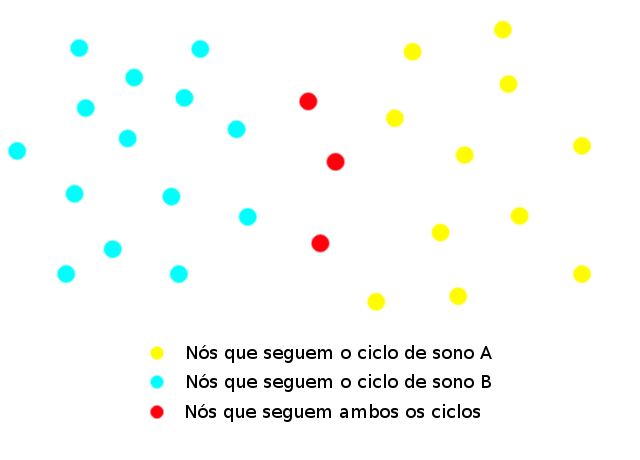
\includegraphics[width=290px,height=180px]{./Pictures/S-MACSynchronization.png}
% SensorNodesScatteredInASensorField.png: 816x1056 pixel, 96dpi, 21.59x27.94 cm, bb=0 0 612 792
% pdfLaTeX aceita figuras no formato PNG, JPG ou PDF
% figuras vetoriais podem ser exportadas para eps e depois convertidas para pdf usando epstopdf
\caption{Exemplo de sincronização de ciclos de atividades com protocolo S-MAC} %legenda
\label{fig:SmacSynch} %rotulo para refencia
\end{figure}
 
 
%\subsection{Transceiver operational states} \cite{Karl2005} pdf-p.47



% sensor-MAC (S-MAC), a MAC protocol
% explicitly designed for wireless sensor networks. While re-
% ducing energy consumption is the primary goal in our design,
% S-MAC also achieves good scalability and collision avoidance
% by utilizing a combined scheduling and contention scheme.
% To achieve the primary goal of energy efficiency, we need to
% identify what are the main sources that cause inefficient use of
% energy as well as what tradeoffs we can make to reduce energy
% consumption.
% 
% We have identified the following major sources of energy
% waste. The first one is collision. When a transmitted packet is
% corrupted, it has to be discarded, and follow-on re-transmis-
% sions increase energy consumption. Collision increases latency
% as well. The second source is overhearing, meaning that a
% node picks up packets that are destined to other nodes. The
% third source is control packet overhead. Sending and receiving
% control packets consumes energy too. The last major source of
% inefficiency is idle listening, i.e., listening to receive possible
% traffic that is not sent. This is especially true in many sensor
% network applications. If nothing is sensed, nodes are in idle
% mode for most of the time. 

%\subsection{Ciclos de Sono} 
 
%Com o objetivo de aumentar o tempo de vida útil das RSSF são utilizados ciclos de sono (\textit{sleep-wakeup cycle} ou \textit{duty cycle}) onde cada nó é ligado apenas por um curto período de tempo (\textit{wakeup}) e então desligado novamente (\textit{sleep}). Devido a utilização desse mecanismo, quando um nó precisa transmitir uma mensagem, ele deve permanecer ligado aguardando que seu destinatário também seja ligado e possa receber essa menságem. A utilização desse ciclos pode aumentar a vida útil das RSSF de poucos dias para vários meses ou mesmo anos dependendo da razão entre o tempo em que o nó permanece ligado e o tempo em que permanece desligado. Segundo \cite{1182838}, os parâmetros chave para caracterizar os ciclos de sono incluem tempo desligado(emph{sleep time}), tempo ligado(\textit{wakeup time}), e a energia consumida durante cada um dos estados (ligado/desligado). 
 
%Além da implementação de ciclos de sono também é possível utilizar ouros mecanismos para, em conjunto com ela, permitir um menor consumo de energia através da eliminação ou redução da ocorrência de outros problemas que podem ocasionar o consumo desnecessário de energia, como \textit{overhearing, protocol overhead, collision, idle lisetening, } etc. 
 
%Esse tipo de controle é realizado por protocolos MAC (Medium Access Control - Controle de Acesso ao Meio). Segundo Karl e Willing os protocolos MAC determinam para um nó os pontos no tempo quando ele pode acessar o meio para tentar trasmitir dados, controles ou pacotes de gerenciamento para outro nó (unicast) ou para um grupo de nós (multicast, broadcast). 
 
\section{Metodologia}

O corrente trabalho pode ser classificado como pesquisa aplicada por tratar com problemas reais. Espera-se como resultado um protocolo que reduza o tempo de transmissão de informação em redes de sensores sem fio sem redução significativa da vida útil da rede. 

É também pesquisa exploratória, pois parte da solução proposta advém da utilização de algoritmos existente para solução de alguns dos problemas (auto organização na formação de estruturas dentro da rede). Possui também características que permitem defini-la como experimental, pois serão utilizadas simulações para verificação e avaliação do protocolo proposto.

Além disso, se caracteriza ainda como pesquisa quantitativa pela utilização de testes, simulações cujos dados quantitativos resultantes serão avaliados com o objetivo de determinar a eficiência do protocolo proposto nesse trabalho.

%\section{Resultados esperados}

Como resultado final desse trabalho, espera-se o desenvolvimento de um protocolo para controle de acesso ao meio (\textit{MAC protocol}) auto-organizado capaz de aumentar a eficiência da rede em termos de latência e economia de energia. 

O protocolo desenvolvido deverá ser capaz de produzir uma organização na rede de sensores de tal forma que seja criada uma sub-estrutura(composta por uma parte dos nós selecionados por um processo de eleição) onde os nós participantes serão sincronizados com uma pequena variação de acordo com o tempo necessário para transmissão de uma mensagem entre dois nós subsequentes. 

Supondo que os nós A, B, C e D façam parte dessa subestrutura, eles seriam sincronizados com um pequeno atraso entre eles, de forma que, na transmissão de uma mensagem de A para D passando por B e C, o tempo de transmissão entre A e B seja menor que o tempo que C leva para acordar depois que A acorda. Espera-se com isso conseguir que o tempo de espera para transmissão de mensagem de cada nó dessa subestrutura seja mínimo. 

Fora dessa subestrutura, a transmissão de mensagens e os ciclos de sono serão controlados por outros protocolos já existentes Considerando que a transmissão de mensagens aconteça entre nós distantes, espera-se que tempo médio de transmissão na rede como um todo também seja reduzido, uma vez que os atrasos causados por tempo de espera para transmissão só ocorram até que mensagem chegue a um nó que pertença à subestrutura formada. 

Como produtos desse trabalho devem ser desenvolvidos:
 
 \subsubsection{Algoritmo de eleição:} esse algoritmo deverá selecionar os melhores candidatos a fazer parte da estrutura com base em seus atributos, por exemplo capacidade de transmissão ou nível de carga da bateria, etc.
 
 \subsubsection{Algoritmo para sincronização:} o algoritmo deverá ser capaz de sincronizar os ciclos de sono dos nós eleitos de forma a porssibilitar a apresentação das características descritas anteriormente.
 
 \subsubsection{Resultados de testes:} apresentação da análise de eficiência do algoritmo com base em simulações computacionais, bem como uma comparação com protocolos já existentes.
 
 \section{Cronograma}
 
\begin{figure}[!htb]
\centering
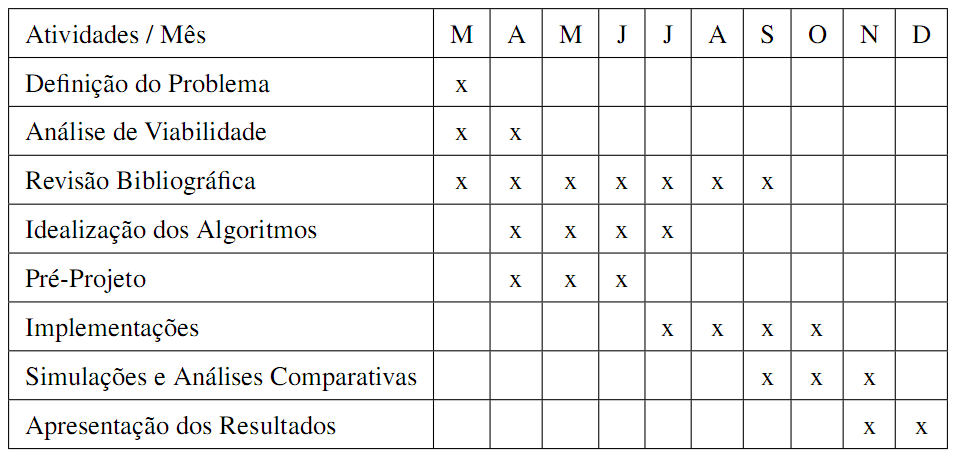
\includegraphics[width=400px,height=180px]{./Pictures/cronograma.png}
% SensorNodesScatteredInASensorField.png: 816x1056 pixel, 96dpi, 21.59x27.94 cm, bb=0 0 612 792
% pdfLaTeX aceita figuras no formato PNG, JPG ou PDF
% figuras vetoriais podem ser exportadas para eps e depois convertidas para pdf usando epstopdf
\caption{Cronograma para o desenvolvimento do projeto} %legenda
\label{fig:cronograma} %rotulo para refencia
\end{figure}
\section{Configurable Sensor MAC ou CS-MAC}

O algoritmo desenvolvido nesse trabalho foi batizado de Configurable Sensor MAC ou Sensor-MAC configurável pois tem como base o algoritmo S-MAC descrito em \citeauthoronline{ye04} (\citeyear{ye04}). Conforme apresentado na sessão ~\ref{sec:smac}, o protocolo S-MAC faz com que cada nó em uma vizinhança siga um mesmo cronograma que determina seus períodos de atividade e inatividade. Com isso, cada nó que deseja transmitir pacotes poderá fazê-lo no momento em que iniciar seu ciclo de atividades sem a necessidade do uso de longos preâmbulos pois o nó receptor iniciará seu ciclo de atividades no mesmo momento.

O protocolo CS-MAC possui os mesmos mecanismos de funcionamento do protocolo S-MAC, podendo ser então considerado uma extensão desse protocolo, pois adiciona a ele mecanismos que permitem que seu funcionamento e configurações sejam alterados por outras camadas da pilha de protocolo, no caso do corrente trabalho, pela camada de aplicação (Sessão ~\ref{sec:applicationLayer}). 

Basicamente, os mecanismos de configuração implementados no protocolo CS-MAC permitem que outra camada possa determinar que o nó siga um cronograma de funcionamento arbitrário especificado por ela com qualquer finalidade. Para o teste dos mecanismos implementados no protocolo CS-MAC, foi implementados na camada de aplicação algoritmos capazes de construir uma ``via de acesso rápido'', por onde os pacotes poderiam trafegar mais rapidamente.

De forma simplificada, os algorítimos implementados são capazes de determinar que uma cadeia de nós situados a uma determinada distância do centro da rede (Figura ~\ref{fig:circularBackbone}) de sensores seja sincronizada de uma maneira tal que, dados os nós A, B e C pertencentes a estrutura, o tempo de transmissão de um pacote de A para C passando por B seria de aproximadamente $2 \cdot T_A$  ($1 \cdot T_A$ = transmissão de A para B, $1 \cdot T_A$ = transmissão B para C) sendo $T_A$ a duração do período de atividade de um nó. 

\begin{figure}[!htb]
\centering
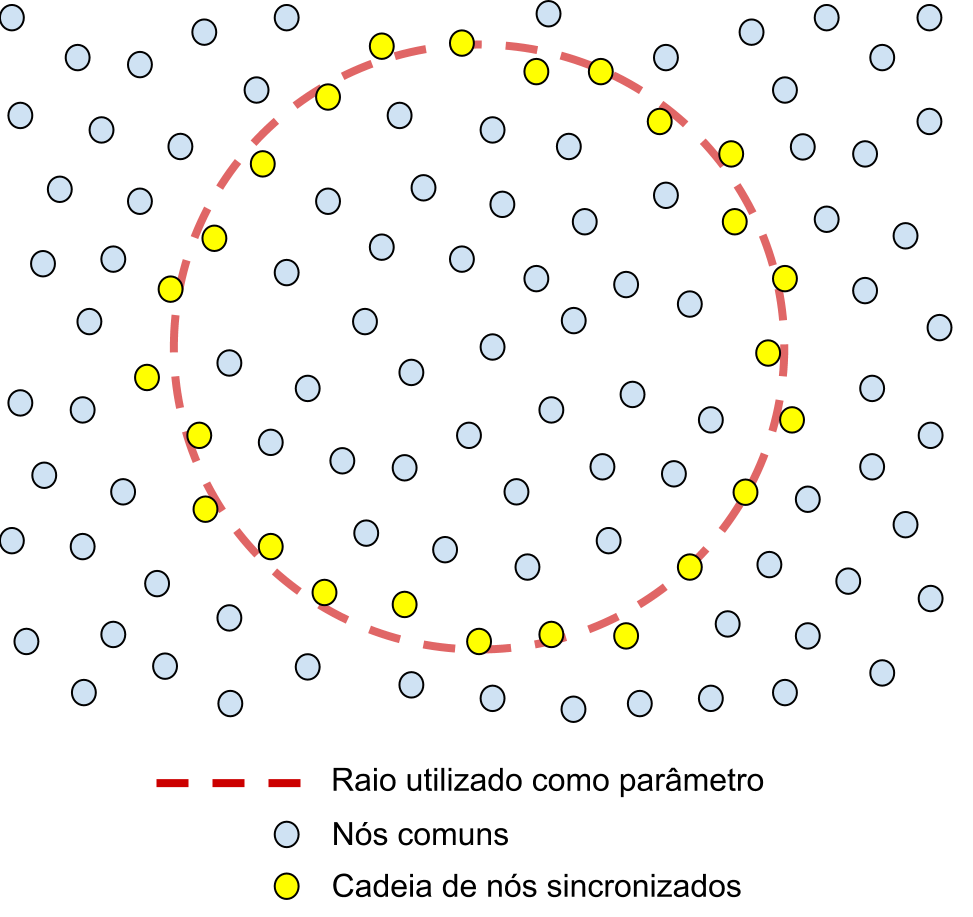
\includegraphics[width=297px,height=280px]{./Pictures/CircularBackbone.png}
% pdfLaTeX aceita figuras no formato PNG, JPG ou PDF
\caption{Cadeia de nós selecionados para sincronização} %legenda
\label{fig:circularBackbone} %rotulo para refencia
\end{figure}

Deve-se notar que não há intervalo entre as duas transmissões. Para que isso seja possível foi determinado que cada nó siga dois cronogramas de atividades distintos sendo que o primeiro cronograma determina um período de atividade no instante $X$ e o segundo determina um período de atividade no instante $X + T_A$. Além disso, primeiro ciclo de atividade de cada nó que participa da cadeia descrita acima deve coincidir com o segundo ciclo de atividades de seu antecessor. A figura ~\ref{fig:backboneSynchronization} abaixo mostra como estão sincronizados os nós do exemplo anterior.

\begin{figure}[!htb]
\centering
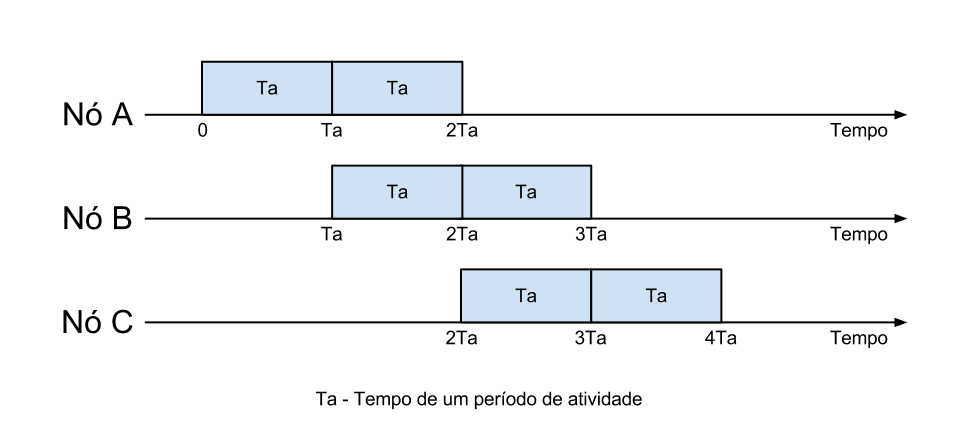
\includegraphics[width=350px,height=163px]{./Pictures/SequencialSynchronization.png}
% pdfLaTeX aceita figuras no formato PNG, JPG ou PDF
\caption{Cronogramas de atividade sincronizados sequencialmente} %legenda
\label{fig:backboneSynchronization} %rotulo para refencia
\end{figure}

As sessões seguintes apresentarão uma descrição mais pormenorizada dos algoritmos utilizados para produzir a organização descrita. Ao final serão também apresentados e discutidos os resultados de simulações realizadas para avaliação dos impactos dessa organização no tempo de transmissão de pacotes entre pontos distantes na rede de sensores.

\section{Algotitmos}

Esse capitulo apresentará os algoritmos utilizados para sincronização dos nós da rede, construção do \emph{backbone} (via de transmissão rápida de pacotes). 
A próxima sessão apresenta o algoritmo selecionado para a sincronização dos nós e razões para a escolha desse algoritmo.

\subsection{Sincronização dos nós}

Como o objetivo do trabalho era o desenvolvimento de um protocolo de comunicação capaz de reduzir o tempo de transmissão de pacotes entre nós distantes na rede e ao mesmo tempo manter o consumo de energia no menos patamar possível, o protocolo S-MAC\cite{ye04} foi selecionado como base para a construção do novo algoritmo. Conforme citado anteriormente na sessão ~\ref{sec:smac}, o algoritmo S-MAC tem como foco o consumo reduzido de energia, além de possuir mecanismos eficientes para redução de perda de pacotes, porém o tempo de transmissão entre nós distantes pode ser muito grande devido ao tamanho dos períodos de dormência dos nós.

No protocolo S-MAC\cite{ye04}, cada nó possui pelo menos uma agenda que determina os momentos em que o rádio-transmissor do nó será ligado (quando o nó poderá enviar e receber pacotes) ou desligado. Essa agenda é compartilhada entre nós vizihos, podendo haver regiões que possuam agendas distintas chamadas \emph{clusters}. Para que seja possível a comunicação entre essas regiões distintas, os nós que estejam no limiar dessas regiões compartilham ambas as agendas, dessa forma podendo enviar e receber pacotes para outros nós de ambas as regiões.

O mecanismo de criação e disseminação de agendas no prodocolo S-MAC funciona de maneira auto-organizada, não necessitando de interferência de agente externo. O algoritmo desenvolvido propõe então uma extensão desse algoritmo de sincronização de modo a disponibilizar mecanismos que permitam a configuração de agendas para os nós de maneira arbitrária, possibilitando que determinados nós sejam acordados em momentos específicos. Através desse mecanismo de configuração, o algoritmo proposto nesse trabalho irá determinar que certos nós sigam agendas específicas que farão com que possuam ciclos de atividade com intervalos muito pequenos entre si, de forma a construis uma cadeia de nós que acordem sequencialmente onde, consequentemente, a transmissão de pacotes por múltiplos nós ocorrerá de maneira muito mais rápida.

Para possibilitar um melhor entendimento funcionamento do protocolo S-MAC e do algoritmo proposto, a sessão seguinte irá apresentar mais detalhes do funcionamento do protocolo S-MAC e do protocolo proposto.

\subsection{Funcionamento do protocolo S-MAC\cite{ye04}}

A partir do momento em que os nós que utilizam o protocolo S-MAC são ligados, eles realizam as seguintes operações:

\begin{itemize}
	\item ``Ouvir'' um ciclo inteiro esperando receber uma agenda que possa seguir.
	\item Caso não receba uma agenda, fará um teste utilizando um valor aleatório para determinar se criará sua propria agenda ou continuará a ``ouvir'' o meio mais um ciclo.
	\item Tendo criado ou recebido uma agenda, irá configurar-se para acordar e dormir de acordo com essa agenda.
\end{itemize}

A partir do momento em que um nó adquire uma agenda seus ciclos de atividade e sono passarão a ser executados repetidamente. Alguns outros mecanismos fazem parte do protocolo, mas um aprofundamento maior foge ao escopo desse trabalho. Mais detalhes sobre o funcionamento do protocolo S-MAC podem ser encontrados em \cite{ye04}. 

Além dos mecanismos providos pelo protocolo S-MAC o novo algoritmo adiciona uma \emph{API } (\emph{Application Program Interface}) para que outras camadas da pilha de protocolo possam determinar uma nova agenda para o nó. Por meio desta, diferentes tipos de configurações para a sincronização entre os nós podem ser determinadas, por exemplo, pela camada de aplicação.

Nesse trabalho, o algoritmo desenvolvido utiliza agentes que percorrem a rede em busca de nós que cumpram determinados requisitos, de modo a formarem uma cadeia circular. Cada um dos nós selecionados é determinado pelo agentes a seguir duas novas agendas uma compartilhada com seu antecessor outra com seu sucessor na estrutura criada, sendo que essas agendas tem um intervalo muito pequeno entre si, suficiente para uma transmissão de pacotes entre os nós. Como resultado do trabalho dos agentes, os nós da cadeia circular estarão sincronizados sequencialmente. Transmissões de pacotes entre nós distantes na rede deverão percorrer essa estrutura visando reduzir o tempo total de transmissão do pacote do nó de origem ao nó destino. As sessões seguintes discutirão os algoritmos utilizados para configuração da rede e disseminação dos agentes.

\subsection{Cálculo da distância ao centro da rede}
\label{sec:calculoDistancia}

Para se determinar a distância de cada nó ao centro da rede é necessário conhecer a sua posição, a maneira mais simples é a utilização de nós que possuam sistema de \emph{GPS} (\emph{Global Positioning System} ou Sistema de Posicionamento Global). Tal sistema permite determinar com precisão a posição a posição de cada nó. Bastaria então que os agentes conhecessem as coordenadas de um ponto no centro da rede para que pudesse determinar se um nó satisfaz ou não os parâmetros que determinam o raio da estrutura circular a ser construída.

Para a utilização de sistema de posicionamento global (GPS) é necessário que cada nó possua \emph{hardware} específico para tal, o que aumenta o seu custo e consumo de energia. Como alternativa ao uso desse sistema é possível realizar o cálculo das distâncias a partir de um no central. Esse nó inicial comunicaria em \emph{broadcast} aos seus vizinhos que ele é o ponto zero. Cada um de seus vizinhos que receba esse pacote poderá determinar sua distância a esse nó central com base na intensidade do sinal recebido.  Cada um desses nós então irá fazer um novo \emph{broadcast} para informar sua distância do centro e assim sucessivamente. 

Para aumentar a precisão do cálculo de sua posição, um nó que já tenha recebido um desses pacotes e receba um novo pacote que determine que uma distância menor ao centro da rede, atualizará seu parâmetro de distância e fará um novo \emph{broadcast} para atualizar seus vizinhos. Isso irá gerar um \emph{flooding} de pacotes na rede, após o qual cada nó conhecerá sua posição e a de seus vizinhos e os agentes poderão utilizar esses valores para a construção da estrutura circular. 

\subsection{Construção do círculo}

Dado que a distância de cada nó em relação ao centro da rede pode ser obtida através das soluções apresentadas na sessão anterior ~\ref{sec:calculoDistancia}, foram utilizados três agentes para a construção da estrutura circular: 

\begin{itemize}
 \item \textbf{\emph{Root finder:}} responsável por percorrer a rede em busca de algum nó que cumpra o requisito de distância do centro da rede (raio do circulo formado). O nó selecionado por esse agente será o nó raiz na estrutura a ser formada. Após encontrar o nó raiz, esse agente irá criar o próximo agente. 
 \item \textbf{\emph{Circle builder:}} responsável por criar as agendas para cada nó (incluindo o nó raiz), determinar qual vai ser o próximo nó que fará parte da estrutura. Ele selecionará vários nós (conforme os mesmos parâmetros do nó anterior) até alcançar algum que já faça parte da estrutura (fechando o círculo), quando então ele criará o próximo agente.
 \item \textbf{\emph{Circle revoker:}} caso o último nó encontrado pelo agente \emph{Circle builder} não coincida com o nó raiz encontrado pelo agente \emph{Root finder}, esse agente será responsável por remover as agendas extras dos nós que foram selecionado, mas não fazem parte do círculo formado (``pontas soltas''), fazendo com que eles voltem a seguir apenas suas agendas originais.
\end{itemize}

\subsection{Roteamento dos pacotes}

Para que a configuração circular formada dentro da rede pelos algoritmos descritos nas sessões anteriores produza efeitos sobre o tempo das transmissões de pacotes dentro da rede, é preciso rotear os pacotes de forma que, caso seja possível, eles sejam encaminhados atrávés da estrutura formada até um ponto próximo do nó destino, quando o pacote deixará a estrutura e será encaminhado ao seu destino através dos mecanismos normais. 

A elaboração de um algoritmo de roteamento de pacotes foge ao escopo desse trabalho. Portanto, com o objetivo de avaliar o desempenho do algoritmo proposto, a determinação do nó receptor em cada transmissão foi feita pelo gerenciador da simulação conforme os seguintes critérios:

\begin{itemize}
\item Caso haja um nó vizinho ao nó transmissor que pertencente à estrutura formada e que esteja mais próximo do nó de destino do pacote do que o transmisso, esse nó será selecionado
\item Caso o critério anterior não seja cumprido, será selecionado como receptor um dos três nós vizinhos mais próximos do nó de destino
\end{itemize}

Utilizando esses critérios foi possível simular um algoritmo de roteamento capaz de fazer com que os pacotes sejam transmitidos através da estrutura circular formada, possibilitanto assim a avaliação de seu desempenho.





%==============================================================================
% Incluindo bibliografia
%\bibliographystyle{plain}             % estilo para labels em numeros
%\bibliographystyle{alpha}             % estilo para labels em iniciais
%\bibliographystyle{abnt-alf}           % estilo para referências usando ABNT, 
\bibliographystyle{abntex2-alf}
                                       % precisa instalar o abntex para usar!!!

%inclui Referências Bibliográficas
\bibliography{Bibliography}


%==============================================================================
% Incluindo anexos numerados com letras maiusculas.
\appendix
% \include{apendice}

%==============================================================================
% Fim do texto
\end{document}
